\documentclass[conference]{IEEEtran}
\IEEEoverridecommandlockouts
\usepackage{cite}
\usepackage{amsmath,amssymb}
\usepackage{graphicx}
\usepackage{booktabs}
\usepackage{multirow}
\usepackage{xcolor}
\usepackage{url}
\usepackage[hidelinks]{hyperref}
\graphicspath{{../feedback/final/figures/}}

\newcommand{\pp}[2]{$#1 \pm #2$}          % difference +- half-width
\newcommand{\Tw}{W}

\begin{document}

\title{Counting the Drops: Deadline-Aware Computing-Aware Traffic Steering under Shared Periodic Telemetry}

\author{\IEEEauthorblockN{Issa Al Sabeh and Hussein Maatouk}
\IEEEauthorblockA{Department of Computer Science, American University of Beirut\\
Beirut, Lebanon}}

\maketitle

\begin{abstract}
Computing-Aware Traffic Steering (CATS) lets network ingresses choose a compute site for each request from metrics that the sites distribute periodically. We study the setting the CATS framework leaves open: several ingresses read the same periodic, byte-budgeted site reports, every request carries a deadline, and an ingress may refuse a request it cannot serve in time. We make three contributions. First, we show that the usual drop-corrected estimate of offered traffic is biased when ingresses drop different shares of their traffic (0.64 to 5.63 times the truth in our runs) and fix it with a 2-byte aggregate drop counter carried in the reports (95\% of estimates within 5\%, against 29\%). Second, in an evaluation frozen in version control before it was run (7,280 simulated runs, 20 seeds, three networks, and a round-robin rival tuned in its own favour), we find that admission control decides most of the deadline success under overload, while steering by measured capacity adds $+9.4$ points when the real capacity differs from the configured one and $+2.0$ points in bursts; in steady load it is level with round-robin plus well-set admission. Third, we confirm in the CATS setting the herd effect known from stale-information load balancing, and draw guidance for how CATS metrics should be distributed. We report one design change made after the first evaluation, its gain ($+0.8$ points) and its cost on fast on/off traffic ($-3.7$ points).
\end{abstract}

\begin{IEEEkeywords}
computing-aware traffic steering, load balancing, stale information, admission control, edge computing, deadlines
\end{IEEEkeywords}

%======================================================================
\section{Introduction}
%======================================================================

Edge applications such as video analytics send a stream of frames that must be processed on a GPU and answered within a deadline. Such a service is usually replicated at several sites of different size and distance. The IETF CATS working group defines how the network edge can steer requests between such sites using both network and computing metrics~\cite{rfc10053,rfc10054}. The framework deliberately stops short of a selection algorithm: it leaves open how metrics are combined, how often they are distributed, and what an ingress should do when every site is busy~\cite{rfc10053,catsmetric}. Requirements in RFC~10054 ask for steering that keeps working with delayed metrics and does not oscillate~\cite{rfc10054}.

This paper studies one concrete version of that open problem. Several ingresses steer frames to a few GPU sites. The sites send the same small report to every ingress every $W$ seconds. Each frame has a deadline of 300~ms, and an ingress may drop a frame at the door when it predicts that no site can answer in time. Three facts make the problem harder than it looks:
\begin{itemize}
\item \emph{The reports are shared and synchronised.} All ingresses see the same numbers at the same moment, so any rule that sends to the apparently best site will send there from every ingress at once.
\item \emph{Dropping hides demand.} A site counts only the frames it receives. Once ingresses start refusing frames, the reports no longer show how much traffic is offered, and each ingress sees only its own refusals.
\item \emph{Configured capacity may be wrong.} Servers fail, are shared, or are misconfigured, and the reports do not say so directly.
\end{itemize}

We built a deadline-aware steering rule for this setting, compared it with eleven baselines in an earlier study, and received the criticism that its contribution was weak: parts were borrowed, it tied with weighted round-robin below capacity, and its estimate of offered traffic was invalid when ingresses drop different shares. This paper is the answer. We fixed the estimator, froze the rule and the evaluation in version control before running it, built the strongest round-robin rival we could from the baselines' own settings, and report every scenario, including those we lose.

\textbf{Contributions.}
\begin{enumerate}
\item \emph{A correct shared estimate of offered traffic} (Section~\ref{sec:est}). The usual correction, arrivals divided by one minus the ingress's own drop share, is biased when ingresses drop different shares, and the bias does not die out. A 2-byte aggregate drop counter in the reports removes it at 4--5\% more telemetry.
\item \emph{Where steering pays under CATS telemetry} (Section~\ref{sec:results}). With a frozen evaluation and a tuned rival, admission control explains most of the deadline success in overload; steering by measured capacity pays when real capacity differs from the configured one and in bursts, and is level with the rival in steady load.
\item \emph{Guidance for CATS metric distribution} (Section~\ref{sec:discussion}). Synchronised shared reports reproduce the herd effect known from stale-information load balancing~\cite{mitz2000}, and recovery after capacity returns is limited by how fast capacity is re-measured.
\end{enumerate}
None of the ingredients is new on its own; Section~\ref{sec:related} states what is known. What we add is their combination in the CATS setting and the evidence. All code, results and freeze notes are public~\cite{repo}.

%======================================================================
\section{Related Work}\label{sec:related}
%======================================================================

\textbf{CATS.} RFC~10053 defines the CATS components and workflow but no selection algorithm or distribution frequency~\cite{rfc10053}; RFC~10054 lists requirements, among them handling stale metrics and avoiding oscillation~\cite{rfc10054}. The metric-definition draft standardises metric levels but leaves aggregation and validity to local policy~\cite{catsmetric}. Proposals such as flow-level load balancing~\cite{catsflowlb} and two-timescale placement~\cite{catsluan} describe mechanisms without an admission algorithm; the latter only says that a controller may reject a request when no candidate fits~\cite{catsluan}. We found no CATS document that evaluates several ingresses acting on the same report.

\textbf{Stale and shared load information.} Mitzenmacher showed that the power of two random choices gives exponential improvements over one choice~\cite{mitz2001}, and that with periodic ``bulletin board'' information, sending to the least-loaded server causes herd behaviour while a little randomness avoids it~\cite{mitz2000}. Dahlin interprets load information by its age~\cite{dahlin2000}. LSQ gives each dispatcher its own local view, refreshed independently~\cite{lsq2020}. Prequal balances on requests in flight and latency obtained by asynchronous probes~\cite{prequal2024}; C3 ranks replicas by observed performance and adds rate control~\cite{c3}. These works do not drop requests and do not reason about a deadline per request.

\textbf{Admission and overload control.} Edge-based distributed admission control is classical~\cite{kelly2000}, and server-driven credits keep tail latency bounded under overload in datacenter RPCs~\cite{breakwater}. Our admission is per frame at the ingress, driven by a predicted deadline miss rather than a delay target, and uses only the shared reports.

\textbf{Positioning.} Table~\ref{tab:matrix} compares the closest approaches. Each ingredient of our rule exists elsewhere; the combination of shared periodic reports at several ingresses, ingress admission, deadline-aware selection and measured capacity, together with a measured estimate of the offered traffic, does not.

\begin{table*}[t]
\centering
\caption{Closest approaches in a CATS-like setting (several ingresses, shared periodic reports, a deadline per request).}
\label{tab:matrix}
\footnotesize
\setlength{\tabcolsep}{4pt}\resizebox{\textwidth}{!}{\begin{tabular}{@{}llccccl@{}}
\toprule
Approach & Information used & Shared info at & Drops at & Deadline in & Measured & Evaluation \\
 & & many ingresses & the door & the decision & capacity & \\
\midrule
Weighted round-robin~\cite{nginxswrr} & configured weights & no telemetry & no & no & no & production use \\
Two choices~\cite{mitz2001} & queues of 2 random servers & fresh info & no & no & no & analysis, simulation \\
Old information~\cite{mitz2000} & periodic bulletin board & yes (herds) & no & no & no & analysis, simulation \\
Stale-load interpretation~\cite{dahlin2000} & stale loads and their age & yes & no & no & no & simulation \\
LSQ~\cite{lsq2020} & own local view per dispatcher & own views & no & no & no & analysis, simulation \\
Prequal~\cite{prequal2024} & async.\ probes: requests in flight, latency & own probes & no & latency-aware & via probes & testbed, production \\
C3~\cite{c3} & per-replica feedback, rate control & yes & backpressure & no & yes & EC2, simulation \\
Liyanage et al.~\cite{liyanage2026} & observed latency per server & own observations & no & SLO risk & via latency & simulation \\
CATS flow-level LB~\cite{catsflowlb} & CATS metrics, weights & yes & no & SLA filter & no & none \\
Two-timescale CATS~\cite{catsluan} & utilisation, link load & not addressed & ``may reject'' & optional & no & supporting only \\
Breakwater~\cite{breakwater} & server queueing delay $\rightarrow$ credits & one server & server side & delay target & n/a & testbed \\
\textbf{This work} & \textbf{shared reports + 2-byte drop counter} & \textbf{yes} & \textbf{yes, per frame} & \textbf{miss risk} & \textbf{yes} & \textbf{7,280 simulated runs} \\
\bottomrule
\end{tabular}}
\end{table*}

%======================================================================
\section{System Model}\label{sec:model}
%======================================================================

\textbf{Sites.} A site $s$ has $c_s$ GPU servers and one first-come, first-served queue. A server processes a frame in 100~ms on average (Gamma-distributed job sizes, squared coefficient of variation 0.25), so a server serves 10 frames/s. A frame whose deadline has passed before service starts is discarded by the site.

\textbf{Ingresses and frames.} $R$ ingresses receive frames as Poisson streams with unequal shares (e.g., 40/30/20/10\%). For each frame, the ingress chooses a site or drops the frame. The end-to-end time is the round trip to the site plus queueing plus processing; the deadline is 300~ms (200~ms in one stress test). Round trips from the first ingress range from 6~ms (nearest edge site) to 120~ms (farthest site); other ingresses are up to 30\% nearer or farther.

\textbf{Telemetry.} Every $W$ seconds, each site sends the same report to every ingress: the number of frames at the site, the time of measurement, and a 4-byte counter of frames that arrived since the last report (62 + 4 bytes). The rules that use our drop counter add 2 bytes per report and 2 bytes per drop count sent (Section~\ref{sec:est}). Reports travel with path delay and may be lost. An ingress knows the configured number of servers per site, the round trips, the reports it received, its own decisions, and the answers to its own frames. It does not see the other ingresses' decisions or the true state of the sites.

\textbf{Metric.} \emph{Deadline success} is the number of frames answered within the deadline divided by all frames generated after the warm-up. A frame dropped at the ingress, discarded at a site, or answered late is a miss. The rejected share is reported next to success so that a rule cannot look good by refusing traffic.

%======================================================================
\section{The Steering Rule}\label{sec:rule}
%======================================================================

The rule runs at every ingress, independently, after each round of reports. It (i) estimates the total offered traffic, (ii) predicts, for each site and each traffic level, how many frames would be late, (iii) plans a split of the total traffic across sites plus a drop share, and (iv) applies the split to its own frames by smooth weighted round-robin~\cite{nginxswrr}. Every ingress computes the plan for the total, so no ingress needs to guess what the others do. We call the frozen version v6.1 and the version with one later change v6.2; v6 is the version criticised in the review.

\subsection{Estimating offered traffic when ingresses drop}\label{sec:est}

Let $A_s$ be the arrivals counted at site $s$ in the last window of length $W$. The total that reaches the sites is $\sum_s A_s/W$, but under overload the offered traffic is larger, because some frames were dropped at the ingresses.

\textbf{The v6 estimate and why it fails.} v6 corrected by the ingress's own drop share $p_i$:
\begin{equation}
\hat{T}_i^{\text{v6}} = \frac{\sum_s A_s / W}{1-p_i}.
\end{equation}
This assumes every ingress drops the same share. It does not: take two ingresses offering 100 frames/s each, where the first drops half and the second none. The sites count 150 frames/s and the truth is 200, but the ingresses estimate $150/0.5 = 300$ and $150/1 = 150$. The simulated v6 gives 299.6 and 149.8.

The error also persists. In a simple model without smoothing, ingress $i$ admits a share $a_i$, believes the total is $A/a_i$, and then admits what fits, $h$; its new share is $a_i h/A$. Every ingress multiplies its share by the same factor $h/A$, so the total admitted converges to what fits while the \emph{ratio} between two ingresses' shares never changes. An ingress that once dropped more keeps over-estimating and keeps dropping more. Measured on the frozen v6, the drop shares of the ingresses differed by up to 63 points (18 points at 130\% load on Beirut), and with reports every 0.5~s the largest ingress estimated 3.1 times the truth on average.

\textbf{The drop counter.} Each ingress counts the frames it drops and, at most every $W/4$ seconds, writes that count (2 bytes) on a frame it sends anyway. Each site adds up the counts it received and reports the sum $D_s$ (2 more bytes). With $D=\sum_s D_s$ and $A=\sum_s A_s$, every ingress uses the same drop share
\begin{equation}
p = \frac{D}{A + D}, \qquad \hat{\lambda}_s = \frac{A_s/W}{1-p}, \qquad \hat{T} = \sum_s \hat{\lambda}_s .
\end{equation}
On the counterexample both ingresses now estimate 198.9 (truth 200). The same share $p$ is applied to every site, since the sites a dropped frame would have gone to are unknown.

\textbf{Smoothing and change tests.} A new value $\lambda_s$ is mixed into the estimate with weight 0.3. A \emph{clear rise}, where the arrivals exceed the arrivals expected under the current estimate, $E_s$, by more than $3\sqrt{E_s}$ (three Poisson standard deviations), is taken at once. v6.2 adds the symmetric test: a \emph{clear fall}, $E_s - A_s > 3\sqrt{E_s}$, is also taken at once. This is the only difference between v6.1 and v6.2 (Section~\ref{sec:v62}).

\subsection{Predicting late frames}

For a site with $n$ frames present, $\ell_s(n)$ is the probability that a new frame finishes after $\tau_s = \delta - \mathrm{RTT}_s$, where $\delta$ is the deadline: the wait for $n-c_s+1$ departures plus the frame's own job, fitted by a Gamma distribution to its mean and variance. The last report of the queue is aged to the present, and through the next interval, with a birth--death model under the planned arrival rate. $r_s(x)$ is the resulting late probability, averaged over four moments of the next interval, if site $s$ receives $x$ frames/s from all ingresses together. A calibration factor $k$ (late share observed in the ingress's own answers divided by late share predicted, over about 100 answers, clipped to $[0.05, 20]$) scales the risk.

\subsection{Planning the split and the drops}

The cost of sending $x$ frames/s to site $s$, in late frames per second, is
\begin{equation}
C_s(x) = x\,\min\{1, k\,r_s(x)\} + \kappa\,\frac{\max\{0,\,n_s(W;x) - n_{s,\text{safe}}\}}{W},
\end{equation}
where $n_s(W;x)$ is the queue at the end of the interval in a fluid model and $n_{s,\text{safe}}$ is the largest queue at which a new frame is still late with probability at most $1/2$. The second term is an externality-inspired backlog penalty: in a single queue at load $\rho$ an extra frame delays about $\rho/(1-\rho)$ later frames, so we set $\kappa = \rho/(1-\rho)$ with $\rho = \min\{0.95, \hat T/\text{capacity}\}$, hence $\kappa \le 19$. Charging every delayed frame as late is an upper bound, so $\kappa$ is a penalty, not a derived conversion; in overload it is the constant 19. The plan solves
\begin{equation}
\begin{aligned}
&\min_{x_1,\dots,x_S,\,x_d} \; \sum_s C_s(x_s) + x_d \\
&\text{s.t.}\;\; \sum_s x_s + x_d = \hat T,\quad 0 \le x_s \le 0.95\,\widehat{\mathrm{cap}}_s ,
\end{aligned}
\end{equation}
where a dropped frame costs exactly one miss. A greedy allocator assigns the traffic in 1\% pieces, each to the site with the lowest incremental cost, or to the drop option when every incremental cost exceeds one miss. Greedy matched the best plan in 99.8\% of 25,671 plans, and replacing it changed success in none of 18 pilot scenarios.

Dropping is allowed only in \emph{overload}, when $\hat T$ exceeds 90\% of the measured capacity, and only after 100 answers have calibrated $k$. Below overload, the plan is used only if it predicts at least 25\% fewer late frames than splitting by capacity; otherwise the capacity split is used.

\subsection{Measuring capacity}

The capacity $\widehat{\mathrm{cap}}_s$ comes from a meter that uses the reports alone: frames served $=$ arrivals minus the change in the queue, counted only while the queue stays at least twice the number of servers for 5~s, so the servers cannot have been idle. A change is accepted when it exceeds half a server plus two standard errors. A site that serves more than its estimate allows is raised at once. A site measured low gets one server back after a quiet spell of $\max(20\,\text{s}, 4W)$; if that was wrong, the next spell is twice as long. The meter needs no new report field.

\subsection{The one change after the first evaluation (v6.2)}\label{sec:v62}

The first evaluation pass (seeds 301--305) showed that v6.1 recovers slowly after a burst. A trace on a pilot seed found two causes: after a burst to 140\% the estimate stayed 1.35 to 1.39 times the truth and was within 6\% only 30~s later, because a fall moved the estimate only 30\% of the way per report; and the capacity meter returned servers one at a time after quiet spells. We addressed the first cause only. Four candidates were compared on pilot seeds 101--105 by a decision rule committed before the pilot runs; the clear-fall test won ($+0.72 \pm 0.17$ points over v6.1 on the 22 Batch~A scenarios, pilot seeds; identical in every steady scenario). v6.2 was then frozen before any of its evaluation runs. The meter's slow return is left as a known limit.

%======================================================================
\section{Evaluation Method}\label{sec:method}
%======================================================================

\textbf{Simulator.} A discrete-event simulator in Python~\cite{repo} models the sites, frames, reports and path delays above. For a given seed, every rule sees exactly the same frames, job sizes, delays, report losses and events (common random numbers), so rules are compared seed by seed. Built-in checks compare the simulator with Erlang-C formulas.

\textbf{Networks} (Table~\ref{tab:nets}). \emph{Beirut} is the network the rule was designed on. The \emph{8-site} network was used earlier to diagnose v6 but never to choose a setting. The \emph{New} network was defined at the v6.1 freeze and never run before; its largest site is far (120~ms, 40\% of the deadline), so capacity alone is no longer a good guide.

\begin{table}[t]
\centering
\caption{Evaluation networks.}
\label{tab:nets}
\footnotesize
\setlength{\tabcolsep}{3pt}
\begin{tabular}{@{}lllll@{}}
\toprule
Network & GPUs per site & Ingresses & $W$ & Run (warm-up) \\
\midrule
Beirut & 2, 4, 8 & 4 & 5 s & 150 s (20 s) \\
8 sites & 1, 2, 2, 3, 4, 5, 7, 8 & 4 & 2 s & 100 s (20 s) \\
New & 2, 3, 5, 6, 8 & 6 & 3 s & 150 s (20 s) \\
\bottomrule
\end{tabular}
\end{table}

\textbf{Scenarios.} \emph{Batch A} (22 scenarios) asks where the gain comes from: steady load from 85\% to 150\%, bursts (140\% for 20~s; on the 8-site network, 5-s bursts at twice the rate), one ingress doubling its traffic, server failures (one of two, four of eight, two of six servers lost for 50--60~s), and wrong weights (the rules are told the large site has 8 servers; 6 work). \emph{Batch B} (14 scenarios) asks whether the estimate holds when ingresses differ: equal and unequal shares, staggered reports, 30\% of reports lost, reports every 0.5 or 1~s, 16 ingresses. \emph{Batch D} (12 scenarios), fixed with v6.2's freeze, lies outside the design range: fast on/off traffic (every 4~s, 2~s at 1.5$\times$ and 2~s at 0.5$\times$ the mean rate) and a 200~ms deadline, each at 95\% and 115\% load on the three networks.

\textbf{Rules.} Besides v6.2, v6.1 and v6, we run: capacity round-robin (RR) with no telemetry; RR with admission (``RR+adm.''), which uses the same reports and the same drop-counter estimate and admits up to a share $U$ of the configured capacity; a deadline-aware static split with the same admission; and two ablations of v6.1 (no backlog penalty; no dropping). RR+adm.\ has two versions. The \emph{frozen rival} ($U = 0.95$, smoothing 0.3) was fixed at the v6.1 freeze. The \emph{tuned rival} ($U = 0.90$, no smoothing) was chosen afterwards on pilot seeds by rules written in advance, as the best setting we could find for RR+adm.; it is the main comparison. All rules that use reports receive the same reports and the same counter, and therefore the same bytes.

\textbf{Protocol.} Seeds 101--105 were used for every design choice. Seeds 301--310 were reserved at the v6.1 freeze; seeds 311--320 were added at the v6.2 freeze and never used before. Rules, scenarios, seeds and the analysis were committed in git with file fingerprints before the runs (tags \texttt{v6.1-frozen} and \texttt{v6.2-frozen}). Differences are paired by seed, with a 95\% Student-$t$ interval (19 degrees of freedom); ``clearly ahead'' means the interval excludes zero. Every scenario is reported and nothing is removed. In total: 7,280 runs (Batch A 4,400; B 1,680; D 1,200), 107.9 million frames in Batch A alone, 13,075 to 40,875 frames per run.

%======================================================================
\section{Results}\label{sec:results}
%======================================================================

\subsection{Where the gain comes from}

Table~\ref{tab:groups} summarises Batch~A by kind of scenario; Fig.~\ref{fig:forestA} shows every scenario. Over all 22 scenarios, v6.2 is ahead of the tuned rival by \pp{2.1}{0.2} points (clearly ahead in 11 scenarios, behind in 3) and ahead of the frozen rival by \pp{5.8}{0.3} (19 ahead, none behind). Mean success is 78.1\% for v6.2, 77.4\% for v6.1, 77.2\% for v6, 76.0\% for the tuned rival, 72.3\% for the frozen rival and 51.8\% for plain round-robin.

\begin{table*}[t]
\centering
\caption{Batch A: difference in deadline success (points), paired by seed, 95\% interval, 20 seeds. In brackets: scenarios clearly ahead / clearly behind / neither. Groups were defined after the first results.}
\label{tab:groups}
\footnotesize
\setlength{\tabcolsep}{4pt}\resizebox{\textwidth}{!}{\begin{tabular}{@{}lccccc@{}}
\toprule
Scenarios ($n$) & v6.2 $-$ tuned rival & v6.1 $-$ tuned rival & v6.2 $-$ v6.1 & v6.1 $-$ frozen rival & v6.2 $-$ frozen rival \\
\midrule
All (22) & \pp{+2.1}{0.2} (11/3/8) & \pp{+1.3}{0.2} (6/6/10) & \pp{+0.8}{0.1} (6/0/16) & \pp{+5.0}{0.3} (19/0/3) & \pp{+5.8}{0.3} (19/0/3) \\
Capacity $\neq$ configured: failures, wrong weights (4) & \pp{+9.4}{1.0} (4/0/0) & \pp{+9.3}{1.0} (4/0/0) & \pp{+0.1}{0.4} (0/0/4) & \pp{+9.3}{1.0} (4/0/0) & \pp{+9.4}{1.0} (4/0/0) \\
Bursts and a surge (6) & \pp{+2.0}{0.2} (6/0/0) & \pp{-0.8}{0.2} (1/3/2) & \pp{+2.8}{0.1} (6/0/0) & \pp{+7.1}{0.2} (6/0/0) & \pp{+9.9}{0.2} (6/0/0) \\
Steady load, 95\% and above (9) & \pp{-0.4}{0.2} (0/3/6) & \pp{-0.4}{0.2} (0/3/6) & \pp{-0.0}{0.0} (0/0/9) & \pp{+3.5}{0.4} (9/0/0) & \pp{+3.5}{0.4} (9/0/0) \\
Steady load, 85--90\% (3) & \pp{+0.1}{0.1} (1/0/2) & \pp{+0.1}{0.1} (1/0/2) & \pp{+0.0}{0.0} (0/0/3) & \pp{-0.1}{0.1} (0/0/3) & \pp{-0.1}{0.1} (0/0/3) \\
\bottomrule
\end{tabular}}
\end{table*}

\begin{figure*}[t]
\centering
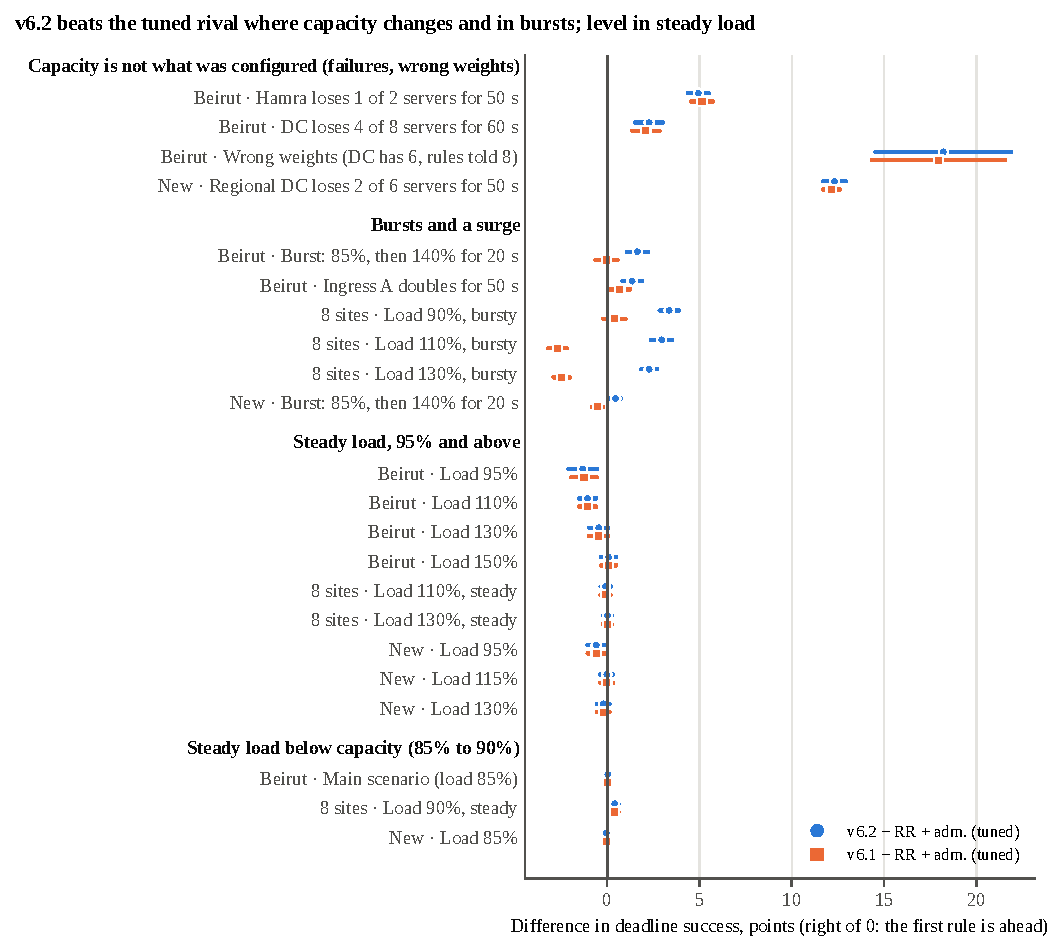
\includegraphics[width=0.80\textwidth]{fig_forest_A.pdf}
\caption{Batch A: v6.2 and v6.1 against the tuned round-robin + admission rival, every scenario (mean difference and 95\% interval over 20 seeds). Groups were defined after the first results.}
\label{fig:forestA}
\end{figure*}

\textbf{Admission is the main lever.} Table~\ref{tab:parts} isolates the parts. With the same round-robin routing, well-set admission raises mean success from 51.8\% to 76.0\%. Our routing without dropping adds \pp{1.4}{0.2} points over round-robin. The backlog penalty adds nothing measurable (\pp{+0.0}{0.1}), nor do the three changes from v6 to v6.1 on success (\pp{+0.1}{0.1}); their purpose is a correct estimate (Section~\ref{sec:resest}). The deadline-aware static split, once tuned, is the capacity split and performs like the frozen rival.

\begin{table}[t]
\centering
\caption{What each part contributes (Batch A, 22 scenarios, points).}
\label{tab:parts}
\footnotesize
\setlength{\tabcolsep}{3pt}
\begin{tabular}{@{}lcl@{}}
\toprule
Comparison & Difference & Shows \\
\midrule
v6.1 $-$ v6.1 without penalty & \pp{+0.0}{0.1} & backlog penalty \\
v6.1 $-$ v6 & \pp{+0.1}{0.1} & changes of v6.1 \\
v6.1 no drop $-$ round-robin & \pp{+1.4}{0.2} & routing alone \\
v6.1 $-$ static split + adm. & \pp{+5.1}{0.3} & static baseline \\
v6.1 $-$ round-robin & \pp{+25.5}{0.4} & floor \\
\bottomrule
\end{tabular}
\end{table}

\textbf{Steering pays when capacity is not what was configured.} In the four failure and wrong-weight scenarios, v6.2 is ahead of the tuned rival in all four, by $+2.3$ (half of a large site lost) to $+18.2 \pm 3.7$ points (wrong weights). The rival admits up to 90\% of a capacity that no longer exists; the meter sees the loss and both steering and admission follow it.

\textbf{In steady load the rival is level or slightly ahead.} At 95\% load and above, v6.2 is behind the tuned rival by \pp{0.4}{0.2} on average, and clearly behind in three scenarios: Beirut at 95\% (\pp{-1.3}{0.8}), Beirut at 110\% (\pp{-1.1}{0.5}) and New at 95\% (\pp{-0.6}{0.5}). Below capacity, all rules are within 0.5 points.

\subsection{The estimate}\label{sec:resest}

Fig.~\ref{fig:estimate} shows the estimate divided by the truth for every ingress of every Batch~B run (1,480 values per rule). With the own-share correction, v6 ranges from 0.64 to 5.63 times the truth and is within 5\% in 29\% of cases. With the drop counter, v6.1 ranges from 0.97 to 1.16 (95\% within 5\%) and v6.2 from 0.95 to 1.04 (100\%). The error of v6 is largest with frequent reports: with reports every 0.5~s on the 8-site network, the ingresses' drop shares ranged from 0.1\% to 77.9\%. Success, however, barely moves (v6.1 $-$ v6: \pp{+0.1}{0.1} in Batch~B), because the total admitted traffic still converges to what fits (Section~\ref{sec:est}). The counter's value is therefore a correct, shared estimate and an even split of the drops between ingresses, not higher success.

\begin{figure*}[t]
\centering
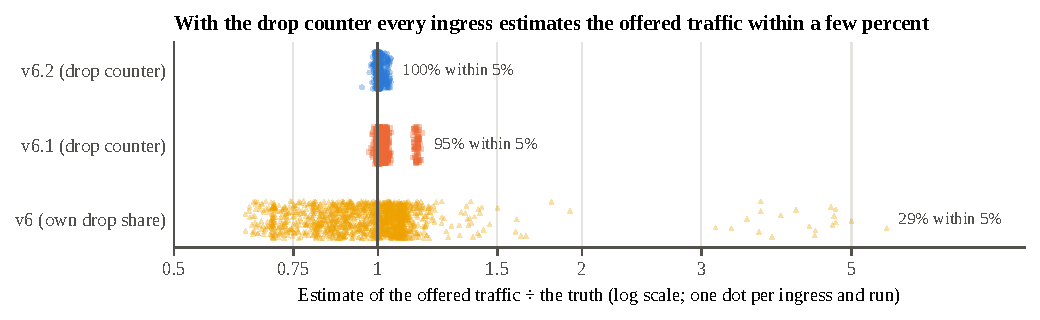
\includegraphics[width=0.78\textwidth]{fig_estimate.pdf}
\caption{Estimate of the offered traffic divided by the truth, every ingress and Batch B run (log scale).}
\label{fig:estimate}
\end{figure*}

\subsection{Recovery after events}

Fig.~\ref{fig:recovery} and Table~\ref{tab:recovery} show the 20~s after each event ends. After the Beirut burst, v6.2 answers 91.9\% of frames in time against 80.7\% for v6.1, and the tuned rival 90.0\%: the clear-fall test removes the slow descent of the estimate. After four DC servers return, both v6.1 and v6.2 stay near 73\% while the rival reaches 94.7\%: the meter still believes the site is half its size and the rule keeps dropping about 21\% of frames. After a small site's or the regional DC's servers return, the order reverses (88.8\% and 87.9\% for v6.2, against 82.1\% and 69.7\% for the rival); the rival likely enters the recovery with the backlog it built at the reduced site.

\begin{figure*}[t]
\centering
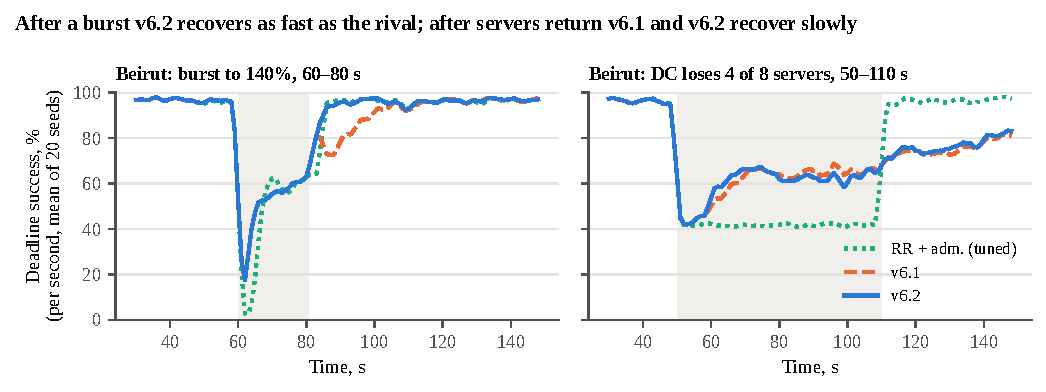
\includegraphics[width=0.78\textwidth]{fig_recovery.pdf}
\caption{Deadline success per second (mean of 20 seeds) around a burst (left) and a server failure and return (right), Beirut network. Shaded: the event.}
\label{fig:recovery}
\end{figure*}

\begin{table}[t]
\centering
\caption{Success / rejected (\%) in the 20 s after the event ends.}
\label{tab:recovery}
\footnotesize
\setlength{\tabcolsep}{3pt}
\begin{tabular}{@{}llccc@{}}
\toprule
Net & Event & v6.2 & v6.1 & Tuned \\
\midrule
Beirut & burst & 91.9 / 5.5 & 80.7 / 18.1 & 90.0 / 7.7 \\
New & burst & 90.6 / 4.8 & 83.5 / 13.2 & 90.8 / 4.8 \\
Beirut & ingress A doubles & 92.1 / 4.4 & 87.4 / 10.8 & 90.3 / 6.3 \\
Beirut & small site, 1 of 2 & 88.8 / 2.6 & 90.3 / 2.1 & 82.1 / 0.1 \\
Beirut & DC, 4 of 8 & 73.5 / 21.1 & 72.7 / 21.6 & 94.7 / 0.1 \\
New & regional DC, 2 of 6 & 87.9 / 1.9 & 87.3 / 2.1 & 69.7 / 0.1 \\
\bottomrule
\end{tabular}
\end{table}

\subsection{Outside the design range}

In Batch~D, v6.2 is ahead of the tuned rival by \pp{6.1}{0.3} points overall (8 scenarios ahead, 2 behind). On fast on/off traffic it is ahead in all six scenarios ($+6.4$ to $+19.4$). The rival rejects far less (6--21\% against 32--47\%), so the frames it admits during the high phases miss their deadline; a likely reason is that our rule also re-plans between reports when the ingress's own arrival rate changes clearly (a burst check), while the rival only reacts at each report. With the 200~ms deadline the picture is mixed: $+4.3$ to $+5.5$ on Beirut, level on the 8-site network, and $-1.3$ to $-1.9$ on the New network, where the far site's 120~ms round trip leaves less than one mean job time within a 200~ms deadline.

\textbf{v6.2's trade-off.} On fast on/off traffic, v6.2 is behind v6.1 by \pp{3.7}{0.3} points on average, and by about 8 points on the 8-site network (44.1\% vs 52.0\% at 95\% load; 33.4\% vs 42.3\% at 115\%). There the traffic changes every 2~s, which is the report interval. The likely mechanism: taking every clear fall at once makes the estimate follow each low phase, so the rule drops too little in the next high phase (it rejects 32.5\% against 36.0\% at 95\% load). v6.2 is thus better in bursts and after them, and worse when the traffic switches at the report timescale. We report both versions rather than replacing v6.1.

\subsection{Telemetry}

Report-based rules receive about 40, 269 and 112 bytes/s per ingress on the three networks. The drop counter costs 4--5\% over v6 (e.g., 40.2 vs 38.3 bytes/s on Beirut), and v6.1, v6.2 and both admission rivals use exactly the same bytes, so no comparison above is bought with extra telemetry. Round-robin uses none.

%======================================================================
\section{Discussion}\label{sec:discussion}
%======================================================================

\textbf{Synchronised reports cause herding.} In an earlier diagnostic on the 8-site network (seeds 201--205, 90\% load, reports every 0.5~s), an LSQ-style rule refreshed by shared reports met 49.3\% of deadlines. Giving each ingress the same information at its own random moment raised this to 85.2\%, while random tie-breaking changed nothing. This is the herd effect of stale bulletin-board information~\cite{mitz2000}, here produced by the CATS distribution model itself, in which every ingress receives the same update at the same time. For CATS this suggests that metric distribution should be desynchronised across ingresses, or that selection rules acting on shared metrics should plan the split of the total traffic, as ours does, rather than pick the apparent best site.

\textbf{A drop counter is cheap and makes the shared estimate correct.} Any CATS deployment that lets ingresses refuse requests hides demand from the sites. Two bytes in the report restore it for every ingress at once, and spread the refusals evenly between ingresses instead of leaving the first ingress to drop the most.

\textbf{Admission first, steering where capacity is uncertain.} Under overload with shared reports, most of the deadline success comes from refusing the right amount of traffic. Steering by measured capacity matters when the real capacity differs from the configured one, and the remaining limit is how fast capacity is re-measured after servers return.

\textbf{Limits.}
\begin{itemize}
\item All results come from a simulator; there is no testbed.
\item Networks have 3 to 8 sites and 4 to 16 ingresses; traffic is Poisson with one on/off pattern; deadlines are 200 and 300~ms; jobs are independent frames, not sessions with affinity.
\item The tuned rival is the best RR+adm.\ setting we found on pilot seeds; a stronger rival may exist.
\item The scenario groups in Table~\ref{tab:groups} were defined after the first results.
\item The main tables hold about 114 intervals at 95\%; about six would exclude zero by chance alone, and no correction for multiple comparisons is applied.
\item The capacity meter returns servers slowly and, in 9 of 110 runs without any failure in an earlier check, measured a site one or two servers too low.
\item v6.2 was designed after the first evaluation pass of v6.1; its own evaluation seeds were unused, but the problem it fixes was seen on evaluation data.
\end{itemize}

%======================================================================
\section{Conclusion}
%======================================================================

We studied deadline-aware site selection when several CATS ingresses share the same periodic, byte-budgeted reports and may refuse requests. A 2-byte aggregate drop counter makes the shared estimate of offered traffic correct, where the usual own-share correction can be off by a factor of five. In a frozen evaluation against a tuned rival, admission control explains most of the deadline success in overload, and steering by measured capacity adds up to 18 points when the real capacity differs from the configured one, while staying level in steady load. The open problems are faster re-measurement of returning capacity and robustness to traffic that changes at the report timescale.

\section*{Reproducibility}
{\raggedright Every number in this paper is computed from the result files in the repository~\cite{repo} by \path{feedback/final/analyze_final.py}; \path{feedback/final/check_final.py} re-runs a sample and checks that reused runs are unchanged. The freeze notes \path{FREEZE_v6.1.md} and \path{FREEZE_v6.2.md} list the parameters, seeds and SHA-256 fingerprints of the frozen files.\par}

\bibliographystyle{IEEEtran}
\bibliography{refs}

\end{document}
